Today's adventure begins as your team's ship launches into space.
Space Fleet has provided you a 
\textbf{Galaxy Map} to guide you on your way.
(Actually, several copies have been provided to you! Take care of
these copies, as you will refer to the Galaxy Map several times 
throughout the adventure.) Each dot on the map refers to a
different solar system, named on the map.

Space Fleet commands you to first visit the four 
\textbf{Core Systems} of
the galaxy. You can recognize a Core System by the fact that
it is located in the middle of a regular polygon
(all sides are the same length) formed by
either three, four, five, or seven other systems. An
example is shown below.

\begin{center}
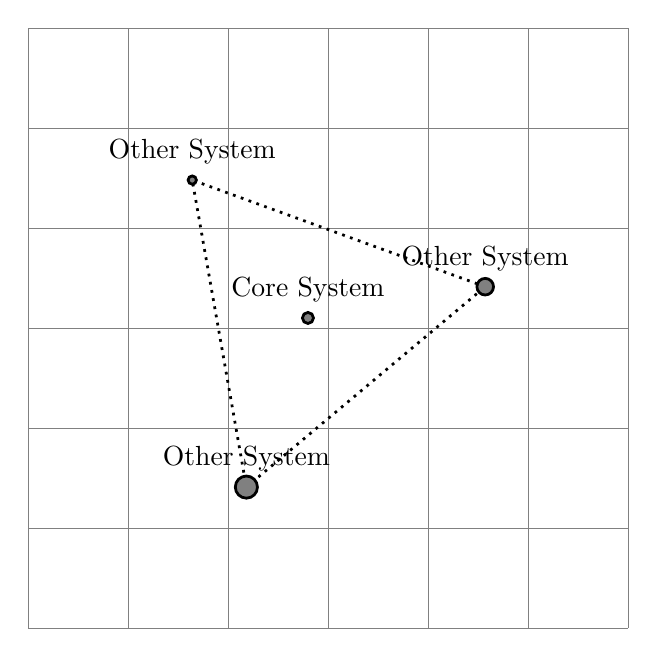
\begin{tikzpicture}[x=0.5in,y=0.5in]
\draw[step=1,gray,very thin] (-3,-3) grid (3,3);
\begin{scope}[
every path/.style={line width=1pt,fill=gray},
shift={(-0.2,0.1)}
]
  %3-gon
  \coordinate (3GonCenter) at (0,0);
  \coordinate (3GonVertex0) at (10:1.8);
  \coordinate (3GonVertex1) at (130:1.8);
  \coordinate (3GonVertex2) at (250:1.8);
  \draw[dotted,fill=none]
    (3GonVertex0) --
    (3GonVertex1) --
    (3GonVertex2) --
    cycle;
  \draw (3GonCenter) node[above=2pt] {Core System} circle (2pt); 
  \draw (3GonVertex0) node[above=2pt] {Other System} circle (3pt); 
  \draw (3GonVertex1) node[above=2pt] {Other System} circle (1.5pt); 
  \draw (3GonVertex2) node[above=2pt] {Other System} circle (4pt);
\end{scope}
\end{tikzpicture}
\end{center}

